\section{Experiments}\label{sec:expts}

\begin{table}[h]
\centering
\small
 \setlength{\tabcolsep}{4pt}
\begin{tabular}{l l l l@{\hskip 0.3cm} l@{\hskip 0.3cm} l l@{\hskip 0.3cm} l l }
\toprule
Dataset & \#folds/ & \#users & \#items & train & test & test & \multicolumn{2}{l}{\#features} \\
              & samples &              &               & \#pairs  & \#pairs & \#scores          & items & users \\
\midrule
Simulation a and b & 25 & 25 & 100 & 900 & 0 & 100 & 2 & 2 \\
Simulation c & 25 & 25 & 100 & 36--2304 & 0 & 100 & 2 & 2\\
\midrule
Sushi A-small & 25 & 100 & 10 & 500 & 2500 & 1000 & 18 & 123 \\
Sushi A & 25 & 100 & 10 & 2000 & 2500 & 1000 & 18 & 123 \\
Sushi B & 25 & 5000 & 100 & 50000 & 5000 & $5\times 1e5$ &  18 & 123 \\
\midrule
UKPConvArgCrowdSample & 32 & 1442 & 1052 & 16398 & 529 & 33 & 32310 & 0
\\ \bottomrule
\end{tabular}
\caption{Summary of datasets showing counts per fold/subsample. 
%For simulations, we generate the subsamples of data independently, 
%for Sushi we select subsamples independently from the dataset.  
%Values for UKPConvArgCrowdSample are means per fold, 
%where the test data in each fold corresponds to a single topic and stance. 
Numbers of features are given after categorical labels have been converted to one-hot encoding, counting
each category as a separate feature.
}
\label{tab:datasets}
\end{table}
Our experiments test key aspects of crowdGPPL: 
 predicting consensus utilities and personal preferences from pairwise labels
 %predicting consensus utilities from noisy crowdsourced preferences
 % in a subjective task; 
 and the scalability of our proposed SVI method.
In Section \ref{sec:exp_synth}, we use simulated data to test the robustness of crowdGPPL
to noise and unknown numbers of latent components.
Section \ref{sec:sushi}
compares different configurations of the model
against alternative methods
using the \emph{Sushi} datasets\footnote{\url{http://www.kamishima.net/sushi/}}~\citep{kamishima2003nantonac}.
Section \ref{sec:exp_scale} evaluates prediction performance and scalability of
 crowdGPPL %to predict both personal and consensus utilities 
in a high-dimensional
NLP task
with sparse, noisy crowdsourced preferences
(\emph{UKPConvArgCrowdSample}\footnote{\url{https://github.com/ukplab/tacl2018-preference-convincing}}, ~\citet{simpson2018finding}).
%Using this latter dataset, we then analyse
%the scalability of our SVI approach. 
Finally, Section \ref{sec:components} evaluates whether crowdGPPL ignores redundant
components.
%when the number of components, $C$,
%is larger than necessary.
The datasets are summarised in Table \ref{tab:datasets}.

%\paragraph{Method Comparison. }

% Ranking-SVM baseline -- only easy to compare in the single user case. My GPPL paper perhaps needs
% this adding in any follow up works.

% Houlsby tests: with/without user features (without is better with few users). + a hierarchical 
% model, BI (multi task preference learning, Birlitiu et al), and the GPPL-joint model. None of 
% these are done at scale, which we can do with our inference method --> *this is a new claim i.e. 
% new empirical results*. They also test a per-user model.

As baselines, we compare crowdGPPL against 
\emph{GPPL},
which we train on all users' preference labels to learn a single utility function,
%and a Gaussian process over the joint feature space of users and items 
%(\emph{joint-GPPL}), as proposed by \citet{guo2010gaussian}.
and \emph{GPPL-per-user},
in which a separate GPPL instance is learned for each user with no collaborative
learning.
We also compare against the \emph{GPVU} model~\citep{khan2014scalable} 
and 
\emph{collabGP} ~\citep{houlsby2012collaborative}.
CollabGP contains parameters for each pairwise label and
 each user, so has a larger memory footprint than our SVI scheme, 
which stores only the moments at the inducing points.
%CollabGP does not learn a consensus or scale parameters $s_c^{(v)}$ and $s_c^{(w)}$,
%and predicts pairwise labels directly rather than utilities that can be used for ranking.
%combines
%matrix factorisation without input features and a separate GP per user. 
%Inference over the latent
%components does not benefit from any item or user features,
%and maximum likelihood steps are used to learn the parameters, rather than applying a fully-Bayesian
%treatment.
% While the original
%implementation used some maximum likelihood steps, we implement GPVU using SVI method 
%to directly compare against crowdGPPL and GPPL-per-user.
% --not quite, as we emulate the ML steps without implementing them exactly.

We test \emph{crowdBT}~\citep{chen2013pairwise} as part of a method for
predicting consensus utilities from crowdsourced pairwise preferences.
CrowdBT models each worker's accuracy, assuming that
the differences between workers' labels are 
due to random errors rather than subjective preferences.
Since crowdBT does not account for the item features,
it cannot predict utilities for items that were not part of the training set.
%and is hence purely an aggregation method.
We therefore treat the posterior mean utilities produced by crowdBT as training labels
for Gaussian process regression using SVI.
We set the observation noise variance of the GP equal to the crowdBT posterior variance
of the utilities 
to propagate uncertainty from crowdBT to the GP. 
This pipeline method, \emph{crowdBT--GP}, 
tests whether it is sufficient to treat annotator differences as noise,
in contrast to the crowdGPPL approach of modelling individual preferences.
%Uncertainty is propagated from crowdBT to the GP through the observation noise variance,
%hence labels that crowdBT has not learned confidently will have less effect on the GP.


We evaluate the methods using the following metrics:
\emph{accuracy (acc)}, which is the fraction of correct pairwise labels;
\emph{cross entropy error (CEE)} between the posterior probabilities over pairwise labels
and the true labels, which captures the quality of the pairwise posterior;
\emph{Kendall's $\tau$}, which evaluates the ranking obtained by sorting items by
predicted utility.

\subsection{Simulated Noisy Data}\label{sec:exp_synth}

\begin{figure}[t]
%\subfloat[Inferring preferences for a single user]{
%\label{fig:simA}
%\includegraphics[width=.35\columnwidth]{../../results/synth_3/single_user/tau_test}
%}
\subfloat[Consensus]{
\label{fig:simB}
\includegraphics[width=.322\columnwidth,clip=true,trim=15 4 13 0]{tau_test}
}
\subfloat[Personal preferences]{
\label{fig:simC}
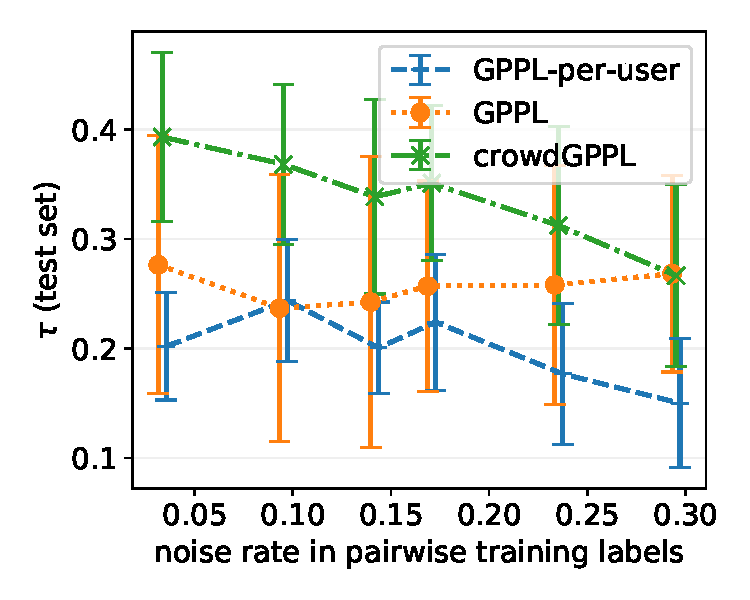
\includegraphics[width=.306\columnwidth,clip=true,trim=30 5 14 0]{tau_test_personal}
}
\subfloat[Latent factors]{
\label{fig:simD}
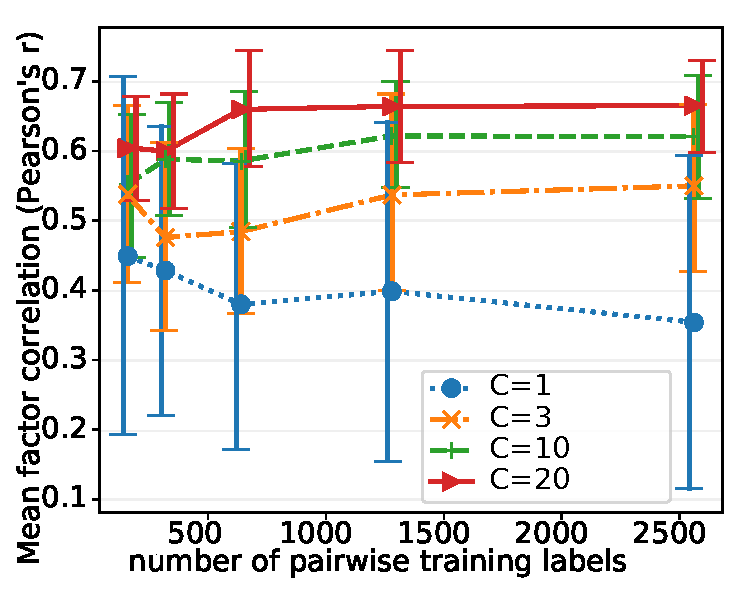
\includegraphics[width=.324\columnwidth,clip=true,trim=8 0 13 0]{num_pairs_r}
}
\caption{Simulations: rank correlation between true and inferred utilities.
(a) \& (b) vary the level of noise in pairwise training labels, (c) varies the number of pairwise training labels. 
}
\end{figure}
First, we evaluate whether crowdGPPL is able to model individual preferences
with varying amounts of labelling noise. 
We set the number of latent components to $C=20$ and all Gamma hyperparameters for crowdGPPL, GPPL and GPPL-per-user 
to $\alpha_0 = 1$, $\beta_0 = 100$.
We use Mat\'ern 3/2 kernels with the length-scale for each dimension of the feature vector, $d$,
chosen by a median heuristic:
\begin{flalign}
 l_{d,\mathrm{MH}} = \mathrm{median}( \{ ||x_{i,d} - x_{j,d}||, 
 \forall i=1,..,N, \forall j=1,...,N\} ).
\end{flalign}
This is a computationally frugal way to choose the length-scales,
%which effectively normalizes the features and 
that has been extensively used in various kernel methods (e.g., ~\citet{bors1996median,gretton2012optimal}).
The SVI hyperparameters were set to 
 $\rho=0.9$, $P_i=1000$ and $\epsilon=1$.
 \citet{hoffman2013stochastic} found that higher values of 
 $\rho$ gave better final results but slightly slower convergence, recommending
 $0.9$ as a good balance across several datasets, 
 and did not find any effect from changing $\epsilon$. 
We follow their recommendations and do not find it necessary to perform further
tuning in our experiments. 
% While we do not find it necessary in our experiments, 
% it is possible to tune $\rho$ and $\epsilon$ using, for example,
% grid search to trade-off between convergence time and maximising the lower bound of the log marginal    
% likelihood, $\mathcal{L}$.
 Both $M$ and $P_i$ are constrained
 %y also found that increasing improves performance, 
 %however this is likely to be constrained 
 in practice by the computational resources available -- we investigate these further in 
 Section \ref{sec:exp_scale}.

 
In simulation (a), to test consensus prediction,
we generate a $20\times 20$ grid of points
and split them into  50\% training and test sets.
For each gridpoint, we generate pairwise labels by drawing from the generative model of crowdGPPL
with $U=20$ users, $C=5$, each $s^{(v)}_c$ set
to random values between 0.1 and 10, and $s^{(w)}_c = 1, \forall c$.
We vary 
%the inverse scale of the consensus function, 
$s^{(t)}$ to control the noise in the consensus function. 
We train and test crowdGPPL with $C=U$ and repeat the complete experiment
$25$ times, including generating new data. 
%for each value of $s^{(t)}$.

Figure \ref{fig:simB} shows that crowdGPPL better recovers the 
consensus ranking than the baselines, even as noise increases, as 
GPPL's predictions are worsened by biased users who deviate
consistently from the consensus. 
For GPPL-per-user, the consensus is simply
the mean of all users' predicted utilities, 
so does not benefit from sharing information between users when training.
For simulation (b), we modify the previous setup 
by fixing $s^{(t)} = 5$ and varying $s^{(v)}_c,\forall c$
to evaluate the methods'
ability to recover the personal preferences of simulated users.
The results in Figure \ref{fig:simC} show that crowdGPPL is able to make better 
predictions when noise is below $0.3$.
% but its benefit disappears when 
%the noise level increases further. 

%In the final simulation, %we evaluate the effect of the quantity of training data 
%with different numbers of latent factors in the generating model.
We hypothesise that crowdGPPL can recover latent components given sufficient training data.
%scenario that would require more training data. 
In simulation (c), we generate data using the same setup as before, 
but fix $s^{(t)} = s^{(v)}_c = s^{(w)} = 1,\forall c$
and vary the number of pairwise training labels 
and the number of true components through
$C_{\mathrm{true}} \in \{ 1, 3, 10, 20\}$.
%We evaluate the correlation between inferred and true user components, 
%we match inferred factors to true factors, 
We match inferred components to the true components as follows:
compute Pearson correlations between each unmatched true component and 
each unmatched inferred component;
select the pair with the highest correlation as a match;
repeat until all true components are matched.
In Figure \ref{fig:simD} we plot the mean correlation between matched pairs of components.
For all values of $C_{\mathrm{true}}$, increasing the
number of training labels beyond $700$ brings little improvement. 
Performance is highest when $C_{\mathrm{true}} = 20$,
possibly because the predictive model has $C = 20$,
so is a closer match to the generating model.
However, %
crowdGPPL is able to recover latent components reasonably well for all
values of $C_{\mathrm{true}}$ given $>500$ labels, despite mismatches between $C$ and $C_{\mathrm{true}}$.
% Does this pose a question: does the mismatch affect the performance? If the correlations
% decrease, it may mean that the model is decomposing a factor into a sum of multiple factors,
% or it may just be unable to learn it. This would need a new experiment: for 700 training pairs,
% how does the accuracy of personalised predictions vary with the number of latent factors?
% I think this needs us to vary C and keep C_true=3, otherwise we don't know whether the 
% performance differences are due to the mismatched no. factors or due to different underlying dataset, i.e. we need to keep the data the same to compare!


\subsection{Sushi Preferences}\label{sec:sushi}

\begin{table}
 \centering
 \small
 \setlength{\tabcolsep}{4pt}
 \begin{tabular}{l l l l@{\hskip 0.5cm} l l l@{\hskip 0.5cm} l l l}
\toprule
& \multicolumn{3}{c}{\textbf{Sushi-A-small}} & \multicolumn{3}{c}{\textbf{Sushi-A}} & \multicolumn{3}{c}{\textbf{Sushi-B}} \\ 
Method & Acc & CEE & $\tau$ & Acc & CEE & $\tau$ & Acc & CEE & $\tau$ \\
\midrule
crowdGPPL & \textbf{.71} & \textbf{.56} & .48 
& .84 & .33 & .79
& .76 & .50 & . 54
 \\
crowdGPPL $\backslash $inducing & .70 & .60 & .45 
& .84 & .34 & .78 
& - & - & - 
\\
crowdGPPL $\backslash  \bs u$ & .70 & .58 & .46 & 
\textbf{.85} & \textbf{.31} & \textbf{.80} 
& \textbf{.78} & .50 & .57 
\\
crowdGPPL $\backslash  \bs u \backslash  \bs x$ & \textbf{.71} & .57 & \textbf{.49} &
\textbf{.85} & .33 & .80 
& .77 & \textbf{.49} & .56 
\\
crowdGPPL $\backslash \bs u,\backslash \bs t$ 
& .68 & .60 & .43 
& .84 & .33 & .80
& .76 & .51 & .58
\\ 
\midrule 
GPPL & .65 & .62 & .31
& .65 & .62 & .31
& .65 & .62 & .31
\\
GPPL-per-user & .67 & .64 & .42
& .83 & .40 & .79 
& .75 & .60 & \textbf{.60} 
\\
collabGP & .69 & .58 & n/a 
& .83 & .35 & n/a
& .76 & \textbf{.49} & n/a
\\
collabGP$\backslash  \bs u$ & .69 & .59 & n/a & .84 & .33 & n/a & .76 & .50 & n/a
\\
GPVU & .70 & .67 & .43 & .72 & .67 & .42 & .73 & .59 & .52
%collabGP$\backslash u, C=50$ & .70 & .58 & n/a & .85 & .33 & n/a & \\
\\ \bottomrule
\end{tabular}
\caption{Predicting personal preferences on \emph{Sushi} datasets,
means over $25$ repeats. 
%CrowdGPPL uses $C=20$ unless otherwise specified.
The standard deviations are $\leq 0.02$ for all accuracies, 
$\leq 0.08$ for all CEE, 
and $\leq 0.03$ for all $\tau$.
For Sushi-B, crowdGPPL, GPPL-per-user and collabGP had runtimes of $~30$ minutes on a 12 core, 2.6GHz CPU server; GPPL required only 1 minute.
 }
\label{tab:sushi}
\end{table}

%We use the \emph{Sushi} datasets
%to compare different variants of crowdGPPL against the baselines and rival methods.
The sushi datasets contain, for each user, a gold standard preference ranking 
of $10$ types of sushi,
from which we generate gold-standard pairwise labels. 
%These labels can be considered noise-free, since
%they are derived directly from the gold standard ranking.  
To test performance with very few training pairs, we obtain \emph{Sushi-A-small}
by selecting $100$ users at random from the complete \emph{Sushi-A} dataset,
then selecting $5$ pairs for training and $25$ for testing per user.
For \emph{Sushi-A}, we select $100$ users at random from the complete dataset, then 
split the data into training and test sets by randomly
selecting $20$ training $25$ test pairs per user. 
For \emph{Sushi-B}, we use all $5000$ workers, and subsample $10$ training and $1$ test pair per user.

We compare standard crowdGPPL with four other variants: 
\emph{crowdGPPL$\backslash$inducing}, which does 
not use the sparse inducing point approximation;
\emph{crowdGPPL$\mathbf{\backslash \bs u}$}, which ignores the user features;
 \emph{crowdGPPL$\mathbf{\backslash \bs u \backslash \bs x}$}, which ignores both user and item features;
 and
 \emph{crowdGPPL$\mathbf{\backslash \bs u \backslash \bs t}$}, which 
excludes the consensus function $\bs t$ from the model as well as the user
features. 
For methods with $\backslash\bs u$, the user covariance matrix, $\bs L$, 
is replaced by the identity matrix, 
and for crowdGPPL$\mathbf{\backslash \bs u \backslash \bs x}$, 
$\bs K$ is also replaced by the identity matrix.
As the user features do not contain detailed, personal information (only 
region, age group, gender, etc.), they are not expected
to be sufficiently informative to predict personal preferences on their own. 
Therefore, for crowdGPPL and crowdGPPL$\backslash$inducing, 
 we compute $\bs L$ for 10 latent components using
 the Mat\'ern 3/2 kernel function 
 and use the identity matrix for the remaining 10.
CollabGP is also tested with and without user features.
We set hyperparameters $C=20$,
$\epsilon=1$, $\rho=0.9$, $P_i=200$ for  \emph{Sushi-A-small} and \emph{Sushi-A},
 and $P_i=2000$ for \emph{Sushi-B},
without optimisation.
For the gamma hyperparameters,  a grid search over 
$\{10^{-1},...,10^3\}$ on withheld user data from \emph{Sushi-A}
resulted in $\alpha_0=1, \beta_0=100$ for GPPL variants, and 
$\alpha_0^{(t)}=1,\beta_0^{(t)}=100$, 
$\alpha_0^{(v)}=1,\beta_0^{(v)}=10$ and
$\alpha_0^{(w)}=1,\beta_0^{(w)}=10$ for crowdGPPL variants.
%All other hyperparameters are the same 
%as for Section \ref{sec:exp_synth}.
The complete process of subsampling, training and testing, was repeated $25$ times
for each dataset.

The results in Table \ref{tab:sushi} 
illustrate the benefit of personalised models over single-user GPPL.
The inducing point approximation does not appear to harm performance of crowdGPPL, but
 including the user features tends to decrease its performance
compared to crowdGPPL$\backslash\bs u$ and crowdGPPL$\backslash\bs u\backslash\bs x$,
except on Sushi-A-small, where they may help with the small amount of training data.
Comparing crowdGPPL$\backslash\bs u$ with crowdGPPL$\backslash\bs u\backslash\bs t$, including the consensus function improves performance modestly.
The strong performance of GPPL-per-user 
suggests that even 10 pairs per person were enough 
to learn a reasonable model for \emph{Sushi-B}.
As expected, the more memory-intensive collabGP performs comparably well to crowdGPPL
on accuracy and CEE but does not provide a ranking function for computing Kendall's $\tau$.
GPVU does not perform as well as other personalised methods on Sushi-A and Sushi-B,
potentially due to its maximum likelihood inference steps.
% The inference method of collabGP did not present practical problems 
% on the Sushi dataset on computer with 16GB RAM, 
% and in fact produces relatively fast run times due to its more efficient implementation using a C library in place of 
% Python. 
The results show that crowdGPPL is competitive despite 
the approximate SVI method, 
so in the next experiment, we test the approach on a larger crowdsourced
dataset where
low memory consumption is required.


\subsection{Argument Convincingness}\label{sec:exp_scale}

% TODO: split the personalised results by no. training examples per worker
% and by model confidence. Does filtering predictions with low confidence estimates
% help? Do workers with more data get better predictions?

\begin{table}
 \centering
 \small
 \setlength{\tabcolsep}{4pt}
\begin{tabular}{ l l l l@{\hskip 1.0cm} l l l@{\hskip 1.0cm} l l l}
\hline
 & \multicolumn{3}{l}{Consensus} & 
 \multicolumn{3}{l}{Personal: all workers} &\multicolumn{3}{l}{$>$50 training pairs} \\
 Method & Acc & CEE & $\tau$ & Acc & CEE & $\tau$ & Acc & CEE & $\tau$ \\ 
  \midrule
 %SVM & .70 & .58 & .31 & .63 & .66 & .31 \\
 %Bi-LSTM & .73 &  .55 & .21 & .64 & .64 & .21 \\
 GPPL  & 
 .77 & .51 & .50 & 
 .71 &  \textbf{.56} & .31 & 
 .72 &  \textbf{.55} & .25 \\ % .71 & .56 & .32 \\ % 
 crowdGPPL & 
 \textbf{.79} & \textbf{.52} & \textbf{.53} & 
 \textbf{.72} & .58 & \textbf{.33} & 
 \textbf{.74} & \textbf{.55} & \textbf{.27}  \\ %.71 & .59 & .32 \\ % now showing workers with > 40 training examples
 crowdGPPL$\backslash \bs t$ & - & - & - &
.68 & .63 & .23 & \textbf{.74} & .57 & \textbf{.27} 
 \\
 crowdBT-GP & .75 & .53 & .45 & .69 & .58 & .30 & .71 & .56 & .23
 \\ \bottomrule
\end{tabular}
%}
\caption{UKPConvArgCrowdSample: predicting consensus, personal preferences for all workers,
and personal preferences for workers with $>$50 pairs in the training set.
%Runtimes on a 12 core, 2.6GHz CPU server were approximately 3 minutes for GPPL and crowdBT-GP, 20 minutes for crowdGPPL.
}
% wilcoxon signed-rank test: crowdGPPL vs. GPPL --> medi. p = 
\label{tab:convarg}
\end{table}
We evaluate consensus learning, personal preference learning and scalability
on an NLP task, namely, ranking arguments by \emph{convincingness}. 
The task requires learning from crowdsourced data, but is not simply an aggregation task as it 
requires learning a predictor for test documents that were not compared by the crowd.
The dataset, \emph{UKPConvArgCrowdSample}, was subsampled by \citet{simpson2018finding}
from raw data provided by \citet{habernal2016argument}, and
contains arguments written by users
of online debating forums,
with crowdsourced judgements of pairs of arguments
 indicating the most convincing argument.
%The task is to quantify how convincing each argument is
%by learning a model from pairwise preference labels obtained from crowdworkers
%on Amazon Mechanical Turk. 
%Each argument is represented by $32,310$ numerical features and the
The data is divided into $32$ folds ($16$ topics, each with 2 opposing stances). For each fold, we train on $31$ folds and test on the remaining fold.
We extend
the task 
%described in \citet{simpson2018finding} 
to predicting both the consensus and personal preferences of individual crowd workers.
%thereby performing a cross-topic evaluation.
%test the ability of the preference learning methods to predict the consensus
 %by training on raw crowdsourced pairwise labels
%for $31$ topics, and testing against the gold pairwise labels and rankings for the
%remaining topic. This` process is repeated for all $32$ topics.
GPPL previously outperformed SVM and Bi-LSTM methods at consensus prediction for \emph{UKPConvArgCrowdSample}~\citep{simpson2018finding}. 
%We compare GPPL with crowdGPPL and also test each method's 
%ability to predict the raw crowdsourced labels, i.e. the individual preference labels
%supplied by each worker.
We hypothesise that a worker's view of convincingness 
depends on their personal view of the subject 
discussed, so crowdGPPL may outperform GPPL and
 crowdBT-GP on both consensus and personal preference prediction.
%We expect crowdGPPL to improve consensus prediction over crowdBT-GP,
%as it accounts for personal biases as well as noisy labels.
%For consensus prediction, crowdBT handles disagreements between workers by treating them 
%as noisy labellers, but we expect that by accounting for 
%for personal biases as well as noise, crowdGPPL may further improve consensus prediction.

The dataset contains $32,310$ linguistic and embedding features
for each document (we use mean GloVe embeddings for the words in each document, see \citet{simpson2018finding}). The high-dimensionality of the input feature vectors requires us to modify the length-scale heuristic for all GP methods,
%of \emph{UKPConvArgCrowdSample}.
as the distance between items grows with the number of dimensions,
which causes the covariance to shrink to very small values. We therefore use
$l_{d,\mathrm{scaledMH}} = 20\sqrt{D} \times l_{d,\mathrm{MH}}$, 
where $D$ is the dimension of the input feature vectors,
and the scale was chosen by comparing the training set accuracy 
with scales in $\{\sqrt{D}, 10\sqrt{D}, 20\sqrt{D}, 100\sqrt{D}\}$.
The hyperparameters are the same as Section \ref{sec:exp_synth} 
except GPPL uses $\alpha_0 = 2$, $\beta_0 = 200$ and
crowdGPPL uses $\alpha^{(t)}_0=\alpha^{(v)}_0=2$, $\beta^{(t)}_0=\beta^{(t)}_0=200$,
$\alpha^{(w)}_0=1$, $\beta^{(w)}_0=10$.
We do not optimise $\alpha_0$, but choose $\beta_0$ by comparing
training set accuracy for GPPL with $\beta_0 \in \left\{2,200,20000\right\}$.
The best value of $\beta_0$ is also used for $\beta^{(t)}_0$ and $\beta^{(v)}_0$, 
then training set accuracy of crowdGPPL is used to select 
$\beta^{(w)}_0 \in \left\{1, 10, 100 \right\}$.
We set $C=50$, $M=500$, $P_i=200$, $\epsilon=10$, and $\rho=0.9$ without optimisation.

Table \ref{tab:convarg} shows that 
crowdGPPL outperforms both GPPL and
crowdBT--GP 
at predicting both the consensus and personal preferences
%pairwise labels
%shown by classification accuracy and cross entropy error,
%and the consensus ranking 
(significant for Kendall's $\tau$ with $p<0.05$, Wilcoxon signed-rank test),
%shown by Kendall's $\tau$ rank correlation.
suggesting that there is a benefit
to modelling individual workers in subjective, crowdsourced tasks. 
%For the personal preference predictions, crowdGPPL also outperforms 
%GPPL.
We also compare against crowdGPPL without the consensus (crowdGPPL$\backslash \bs t$)
and find that including $\bs t$ in the model improves personalised
predictions. This is likely because many workers have few training pairs, 
so the consensus helps to identify arguments that are commonly considered very poor or very
convincing.
Table \ref{tab:convarg} also shows that for
workers with more than 50 pairs in the training set,
accuracy and CEE improve for all methods but
$\tau$ decreases,
suggesting that some items may be ranked further away from their correct ranking 
for these workers. It is possible that workers who were willing to complete more
annotations (on average 31 per fold)
deviate further from the consensus, and crowdGPPL does not fully capture
their preferences given the data available.

\begin{figure}
\centering
\subfloat[Varying $M$]{
\label{fig:M}
 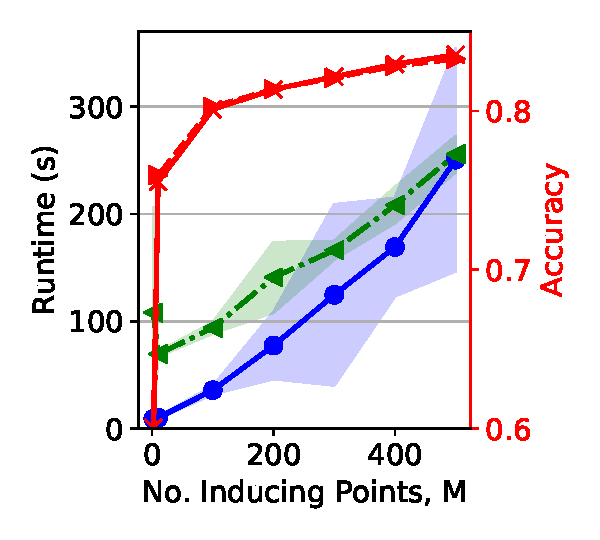
\includegraphics[clip=true,trim=9 0 55 0,width=.24\columnwidth]{num_inducing_32310_features}
}
\subfloat[Varying $P_i$   \hspace{0.5cm}]{
\label{fig:P_i}
 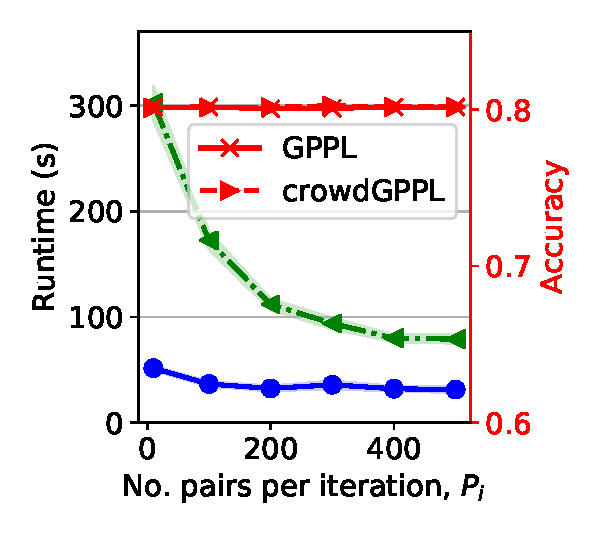
\includegraphics[clip=true,trim=60 2 9 0,width=.236\columnwidth]{P_i_32310_features}
}
\subfloat[Varying $N$]{
\label{fig:Ntr}
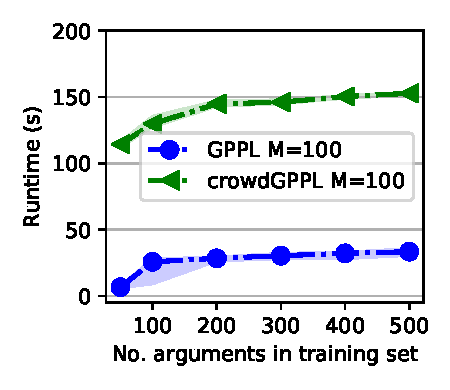
\includegraphics[clip=true,trim=9 0 10 0,width=.24\columnwidth]{num_arguments}
}
\subfloat[Varying $P$ ]{
\label{fig:Npairs}
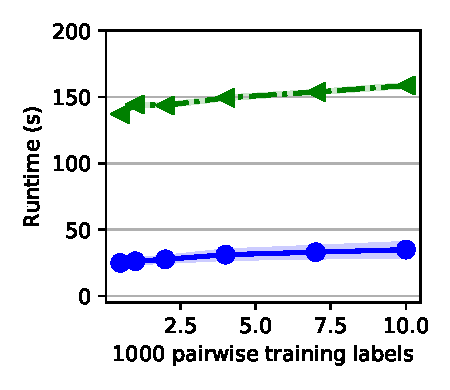
\includegraphics[clip=true,trim=26 0 10 0,width=.22\columnwidth]{num_pairs}
}
\caption{
    Wall-clock times for training+prediction of consensus utilities for arguments 
    in the training folds of
    UKPConvArgCrowdSample. CrowdGPPL was run with $C=5$. In (b), (c) and (d),  $M=100$.
    Lines show means over 32 runs,
     bands indicate 1 standard deviation (mostly very little variation between folds).
}
\end{figure}
We examine the scalability of our SVI method by evaluating GPPL and crowd-GPPL with
different numbers of inducing points, $M$,
and different mini-batch sizes, $P_i$.
%Here, we fix $C=5$ and keep other model hyperparameters 
%and experimental setup the same as for Table \ref{tab:convarg}. 
Figure \ref{fig:M} shows the trade-off between
runtime and training set accuracy as an effect of choosing $M$. 
Accuracy levels off as $M$ increases,
while runtime continues to increase rapidly in a polynomial fashion.
Using inducing points can therefore give a large improvement in runtimes 
with a fairly small performance hit.
Figure \ref{fig:P_i} demonstrates that
smaller batch sizes do not negatively affect the accuracy,
although they increase runtimes as more iterations are required for convergence.
The runtimes flatten out as $P_i$ increases, so we recommend choosing $P_i\geq 200$
but small enough to complete an iteration rapidly with the computational resources available.
Figures \ref{fig:Ntr} and \ref{fig:Npairs} show runtimes as a
function of the number of items in the training set, $N$,
and the number of pairwise training labels, $P$, respectively (all other settings remain as in Figure \ref{fig:M}).
In both cases, the increases to runtime are small, despite the growing dataset size.

\subsection{Posterior Variance of Item Components}
\label{sec:components}

\begin{figure}
\centering
\subfloat[\emph{UKPConvArgCrowdSample}]{
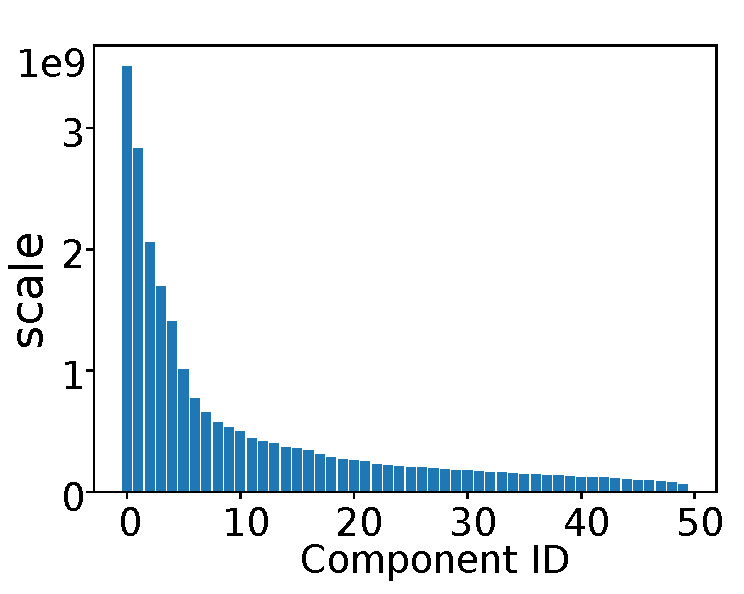
\includegraphics[trim=0 10 0 20,clip=true,width=.24\textwidth]{conv_factor_scales2}
\hspace{1cm}
}
\subfloat[\emph{Sushi-A}]{
\hspace{1cm}
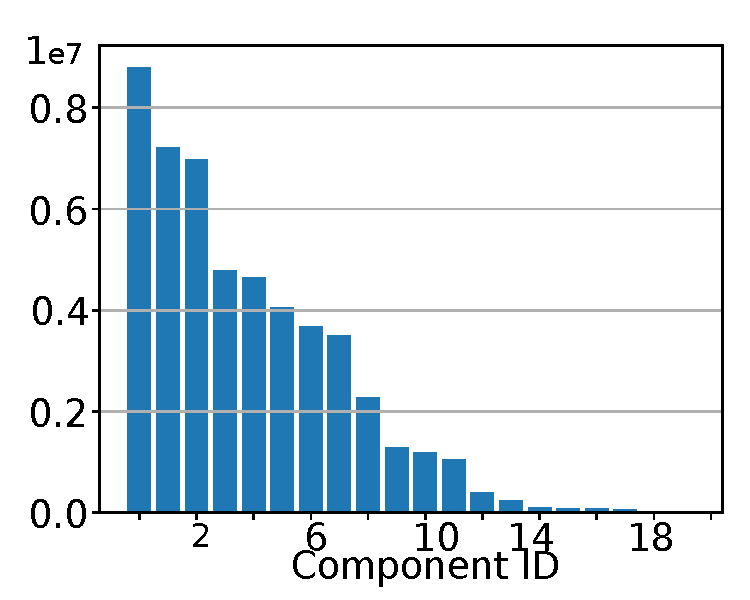
\includegraphics[trim=10 5 0 20,clip=true,width=.23\textwidth]{sushi_factor_scales2}
}
\caption{
Latent component variances, $1/(s^{(v)}_c * s^{(w)}_c)$ in crowdGPPL, means over all runs.
}
\label{fig:latent_factor_variance}
\end{figure}
We investigate how many latent components were actively used by 
 crowdGPPL on the \emph{UKPConvArgCrowdSample} and \emph{Sushi-A} datasets.
Figure \ref{fig:latent_factor_variance}
plots the posterior expectations of the inferred scales, $1/(s^{(v)}_c * s^{(w)}_c)$, for the latent item 
 components. 
 The plots show
that many factors have a relatively small variance and therefore do not contribute 
to many of the model's predictions. This indicates that 
our Bayesian approach will only make use of components that are supported by the data, 
even if $C$ is is larger than required.

